\documentclass[conference]{IEEEtran}

\usepackage{amsmath,amssymb,amsfonts}
\usepackage{graphicx}
\usepackage{textcomp}
\usepackage{xcolor}
\usepackage{booktabs}
\usepackage{url}
\usepackage{cite}
\usepackage{multirow}
\usepackage{array}
\usepackage[table]{xcolor}
\usepackage{hyperref}

\definecolor{headerblue}{RGB}{52,90,150}
\definecolor{groupgray}{RGB}{230,230,230}
\definecolor{rowalt}{RGB}{245,248,255}

% Allow more figures per page in two-column mode
\setcounter{dbltopnumber}{4}
\renewcommand{\dbltopfraction}{0.99}
\renewcommand{\textfraction}{0.01}
\renewcommand{\floatpagefraction}{0.8}
\renewcommand{\dblfloatpagefraction}{0.8}

\def\BibTeX{{\rm B\kern-.05em{\sc i\kern-.025em b}\kern-.08em
		T\kern-.1667em\lower.7ex\hbox{E}\kern-.125emX}}

\begin{document}

\title{Multi-Agent Explainable AI Text Classification: A Pattern Recognition Approach
	with Classical and Transformer-Based Models\\
}

\author{\IEEEauthorblockN{Oruç Çakır}
	\IEEEauthorblockA{\textit{Department of Computer Engineering}\\
		\textit{TOBB University of Economics and Technology}\\
		Ankara, Turkey \\
		Student ID: 211101023 \\
		oruccakir@etu.edu.tr}
}

\maketitle

\begin{abstract}
This paper addresses the following pattern recognition research question: can a
multi-agent architecture effectively route and classify multilingual text, and how do
classical pattern classifiers compare to transformer-based models in Macro-F1
and feature interpretability? I designed a three-agent system in which one agent routes
inputs, one classifies, and one generates SHAP/LIME explanations. I trained and
benchmarked the pipeline on four datasets: IMDB (binary sentiment, English), AG News
(4-class topic, English), Turkish Sentiment (3-class sentiment), and Turkish News
(7-class topic); full benchmark results are available at the project repository. I focus
the deep analysis on Turkish Sentiment (440K short texts), a challenging imbalanced
scenario. I compare seven classical classifiers (Naive Bayes, SVM, Logistic Regression,
Random Forest, KNN, Decision Tree, XGBoost) and BERTurk, using TF-IDF with L2
normalization on a 50K stratified subsample. BERTurk achieves Macro-F1 = 0.9298, while
SVM is the strongest classical model at Macro-F1 = 0.8768, a gap driven primarily by
the imbalanced \textit{negatif} minority class (11.6\%), not overall accuracy. My
10-run statistical analysis confirms SVM significantly outperforms all classical
alternatives.
\end{abstract}

\begin{IEEEkeywords}
text classification, pattern recognition, feature extraction, multi-agent systems,
SHAP, LIME, BERTurk, Turkish NLP, class imbalance
\end{IEEEkeywords}

% ============================================================
\section{Introduction}
\label{sec:introduction}
% ============================================================

Automatic text classification is a fundamental pattern recognition problem. Given a
feature representation of a text document, the task is to assign it to one of a
predefined set of categories. The central challenge is not only to achieve high accuracy
but also to understand \textit{why} a classifier assigns a given label, the
interpretability dimension of pattern recognition.

Classical pattern recognition classifiers such as SVM, Naive Bayes, and Logistic
Regression operate on hand-crafted feature spaces (e.g., TF-IDF vectors), making their
decision boundaries geometrically interpretable. In contrast, transformer-based models
like BERT~\cite{b2} learn contextual representations that capture morphological and
semantic nuance, at the cost of interpretability. On balanced datasets their Macro-F1
advantage over SVM is only 1.2--1.9 points; the gap widens to 5.3 points when class
imbalance is present. Explainability tools (SHAP~\cite{b4} and LIME~\cite{b5})
bridge the interpretability gap by providing post-hoc, model-agnostic feature attributions.

The central research question of this project is:
\begin{quote}
\textit{``Can a multi-agent architecture effectively route and classify multilingual
text, and how do classical pattern classifiers compare to transformer-based models in
terms of Macro-F1 and interpretability across diverse datasets?''}
\end{quote}

I built a three-agent pipeline and trained it on four datasets: IMDB, AG News, Turkish
Sentiment, and Turkish News. Section~\ref{sec:dataset}--\ref{sec:results} focus the
deep pattern recognition analysis on Turkish Sentiment, the most challenging scenario
due to class imbalance and Turkish agglutinative morphology. Summary results for all
four datasets are in Appendix~B; full per-model figures are at the project repository.

The main contributions are:
\begin{itemize}
	\item Training and benchmarking of eight classifiers (seven classical + BERTurk)
	      across four multilingual datasets (IMDB, AG News, Turkish Sentiment, Turkish
	      News); detailed pattern recognition analysis focused on the imbalanced
	      Turkish Sentiment task.
	\item A 10-run statistical experiment confirming SVM significantly outperforms
	      all classical alternatives ($p < 0.0001$), with analysis of why linear
	      margin classifiers suit sparse TF-IDF feature spaces.
	\item A three-agent modular pipeline integrating multilingual routing and
	      on-demand SHAP/LIME explainability for all model types.
\end{itemize}

The rest of this paper is organized as follows:
Section~\ref{sec:related_work} reviews related work.
Section~\ref{sec:architecture} describes the system architecture.
Section~\ref{sec:dataset} presents the dataset and feature analysis.
Section~\ref{sec:models} describes the models.
Section~\ref{sec:results} presents results.
Section~\ref{sec:conclusion} concludes the paper.

% ============================================================
\section{Related Work}
\label{sec:related_work}
% ============================================================

\subsection{Pattern Recognition for Text Classification}

Text classification is a core pattern recognition problem. Duda, Hart, and
Stork~\cite{b_duda} establish the theoretical foundations: feature extraction,
classifier design, and the bias--variance trade-off. In text domains, Naive Bayes,
SVM, and Logistic Regression remain competitive baselines because TF-IDF vectors
are high-dimensional and sparse, conditions that favor linear classifiers
over complex non-linear models~\cite{b_duda}.

\subsection{Deep Learning and Pre-trained Language Models}

BERT~\cite{b2} changed NLP by introducing bidirectional context. Schweter~\cite{b7}
released BERTurk, pre-trained specifically on Turkish text. Minaee et al.~\cite{b10}
survey deep learning methods for text classification, confirming transformers outperform
classical models on large datasets but not always on small or class-imbalanced ones.

\subsection{Explainable AI for NLP}

Lundberg and Lee~\cite{b4} proposed SHAP using game-theoretic Shapley values.
Ribeiro, Singh, and Guestrin~\cite{b5} introduced LIME, which perturbs inputs to fit
local linear surrogates. Both methods are model-agnostic and applicable to the full
spectrum from Naive Bayes to transformers.

\subsection{Turkish NLP}

Turkish's agglutinative morphology creates a very large vocabulary, challenging
classical bag-of-words models. BERTurk~\cite{b7} addresses this via subword tokenization
pre-trained on Turkish corpora. Multi-agent systems~\cite{b_wj} provide a modular
framework for combining multiple specialized classifiers.

% ============================================================
\section{System Architecture}
\label{sec:architecture}
% ============================================================

My system has three agents that collaborate as shown in Fig.~\ref{fig:architecture}.

\textbf{Agent 1 (Intent Classifier).} Takes raw user input and uses an LLM to detect
language (English or Turkish) and domain (sentiment or news), routing to the correct
dataset-model pair.

\textbf{Agent 2 (Classification Agent).} Loads the selected model and returns the
predicted label with confidence scores for all classes.

\textbf{Agent 3 (XAI Agent).} Generates SHAP and LIME explanations for any classifier
via a unified \texttt{predict\_proba} wrapper, making explanations comparable across
model types.

\begin{figure}[htbp]
	\centerline{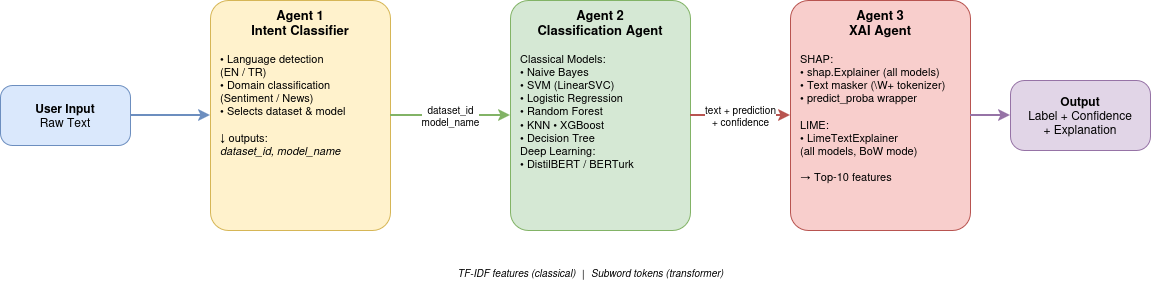
\includegraphics[width=\columnwidth]{architecture.png}}
	\caption{Three-agent pipeline. Agent~1 routes inputs by language and domain.
	         Agent~2 classifies using any of six models. Agent~3 explains predictions
	         with SHAP and LIME.}
	\label{fig:architecture}
\end{figure}

% ============================================================
\section{Dataset: Turkish Sentiment Analysis}
\label{sec:dataset}
% ============================================================

\subsection{Data Source}

I use the Turkish Sentiment dataset~\cite{b_trsentiment} available on HuggingFace.\footnote{\path{winvoker/turkish-sentiment-analysis-dataset}}
It contains product and social media reviews in Turkish with three sentiment
classes (pozitif, notr, negatif) and comes with predefined train/test splits, making
it a standard benchmark for Turkish multi-class sentiment classification.

\subsection{Dataset Description}

The dataset contains 440,679 training samples and 48,965 test samples. Texts are short
(average $\approx$140 characters, $\approx$35 subword tokens). For computational
feasibility, I use a stratified subsample of 50,000 training samples and a 10,000-sample
stratified test subset for evaluation.\footnote{The full 48,965-sample test set was used
for preliminary checks; all reported numbers use the 10,000-sample stratified subset for
reproducibility with seed 42.}

\subsection{Preprocessing Stages}

I apply the following preprocessing steps:
(1) URL removal via regex; (2) lowercase conversion; (3) punctuation removal, preserving
Turkish characters (ç, ğ, ı, ö, ş, ü); (4) Turkish stopword filtering using a 76-word
list; (5) minimum word-length filter ($\geq$2 characters). I do not apply stemming or
lemmatization; TF-IDF handles vocabulary variation statistically.

\subsection{Feature Descriptions}

I use TF-IDF vectorization~\cite{b_tfidf} to produce a 30,000-dimensional sparse feature vector per
sample. The TF-IDF weight $w_{t,d}$ of term $t$ in document $d$ is:
\[
w_{t,d} = (1 + \log \text{tf}_{t,d}) \cdot \log \frac{N}{\text{df}_t}
\]
where $\text{sublinear\_tf=True}$ applies the log transform, $N$ is the number of
documents, and $\text{df}_t$ is the document frequency of term $t$. Unigrams and
bigrams (\texttt{ngram\_range=(1,2)}) are included to capture negations and compound
sentiment expressions.

\subsection{Feature Selection and Adjustment}

I filter the vocabulary with \texttt{min\_df=3} (removing features appearing in fewer
than 3 documents) and \texttt{max\_df=0.95} (removing overly common stop-phrases).
This gives me a final vocabulary of 30,000 features, balancing informativeness and
computational cost.

\subsection{Other Problem-Specific Processing}

Turkish agglutinative morphology means that a single root word can generate hundreds
of inflected forms (e.g., \textit{gel}, \textit{geldi}, \textit{gelmedi},
\textit{gelmeyecekti}). Rather than applying a morphological analyzer, I rely on the bigram vocabulary to
capture common suffix co-occurrences, giving implicit morphological coverage at
lower computational cost.

\subsection{Class Data Distribution}

Table~\ref{tab:class_dist} shows the training class distribution. The dataset is
significantly imbalanced: \textit{negatif} comprises only 11.6\% of samples, creating
a minority-class problem. This imbalance motivates the use of Macro F1 as the primary
evaluation metric, since accuracy can be inflated by the majority class (pozitif: 53.5\%).
I did not apply SMOTE or class-weighted loss in this experiment, which I acknowledge
as a limitation.

\begin{table}[htbp]
	\caption{Turkish Sentiment Class Distribution (Training Set)}
	\label{tab:class_dist}
	\begin{center}
		\footnotesize
		\renewcommand{\arraystretch}{1.2}
		\setlength{\tabcolsep}{8pt}
		\begin{tabular}{lrr}
			\toprule
			\rowcolor{headerblue}
			\color{white}\textbf{Class} & \color{white}\textbf{Count} & \color{white}\textbf{\%} \\
			\midrule
			pozitif   & 235,949 & 53.5\% \\
			notr      & 153,825 & 34.9\% \\
			negatif   &  50,905 & 11.6\% \\
			\midrule
			\textit{Total} & \textit{440,679} & \\
			\bottomrule
		\end{tabular}
	\end{center}
\end{table}

\subsection{Data Normalization}

I apply L2 normalization to every TF-IDF vector via \texttt{norm='l2'} in
\texttt{TfidfVectorizer}, so that each sample vector has unit Euclidean norm. This
is not a separate pipeline step but is built into the vectorizer. L2 normalization is
critical for SVM and KNN: for LinearSVC, it ensures that the decision boundary margin
is measured in consistent geometric units regardless of text length; for KNN with cosine
distance, it makes cosine similarity equivalent to inner product, enabling efficient
computation. Without normalization, longer reviews would dominate shorter ones purely due
to higher cumulative TF-IDF weights.

\subsection{Visual Representation of Feature Space}

To visualize the feature space, I applied PCA to 50 dimensions and then t-SNE~\cite{b_tsne}
(\texttt{perplexity=30}, \texttt{random\_state=42}) to 2,000 stratified test samples,
as shown in Fig.~\ref{fig:tsne}. The three classes form partially
overlapping regions, with \textit{pozitif} and \textit{notr} substantially mixed,
reflecting the semantic ambiguity between neutral and positive Turkish text. The
\textit{negatif} class is more separated but still overlaps with \textit{notr}, which
explains the lower recall for the negatif class across all models.

\begin{figure}[htbp]
	\centerline{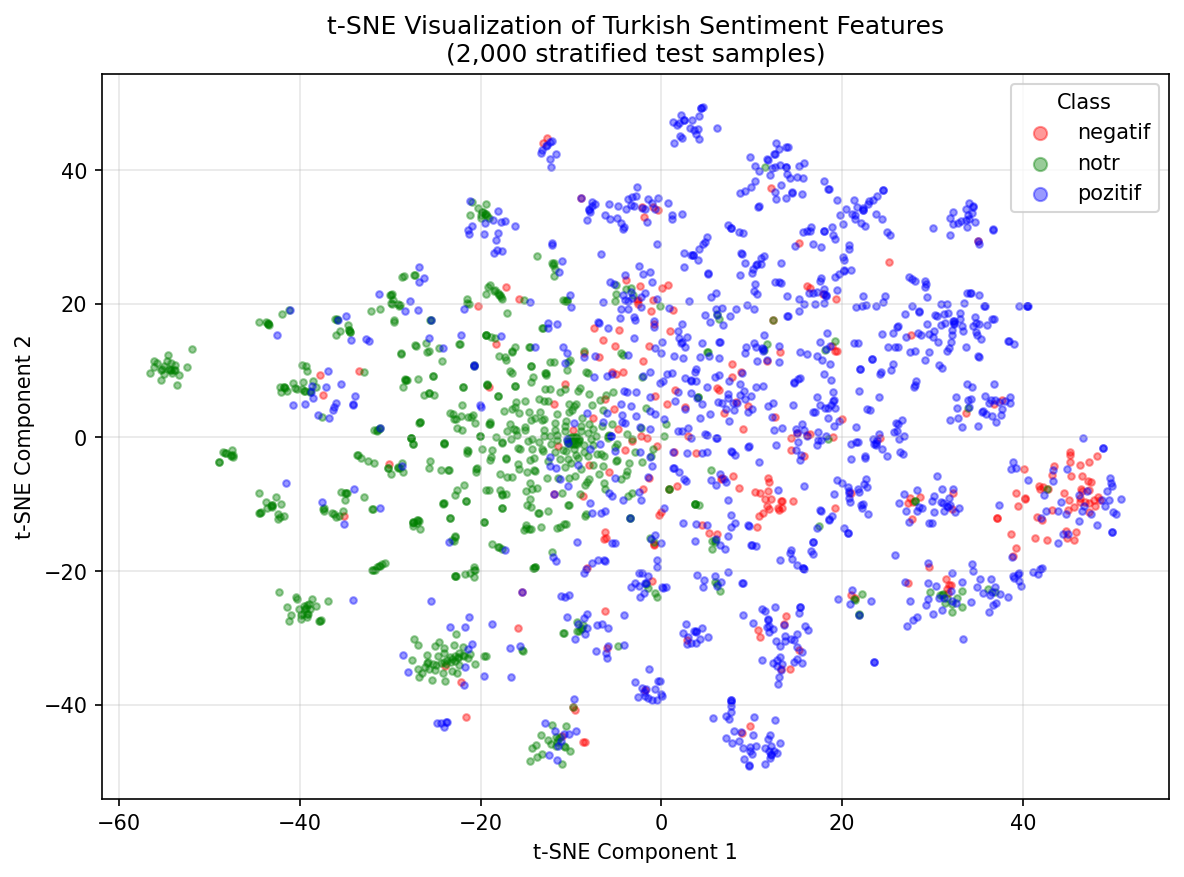
\includegraphics[width=\columnwidth]{turkish_sentiment/tsne_2d.png}}
	\caption{t-SNE 2D projection of 2,000 test samples (PCA-50 + t-SNE). Partial
	         class separation is visible, with negatif (red) forming a loose cluster
	         away from pozitif (blue) but overlapping with notr (green).}
	\label{fig:tsne}
\end{figure}

\subsection{Relationships Between Features}

I extracted the top-10 TF-IDF features per class from the SVM's LinearSVC
\texttt{coef\_} attribute and list them in Table~\ref{tab:top_features}. These weights are directly
interpretable as per-class discriminative scores. The pozitif features
(\textit{harika}, \textit{mükemmel}, \textit{güzel}) are strong positive sentiment
words. The negatif features (\textit{berbat}, \textit{kötü}, \textit{rezalet},
\textit{iade}) clearly indicate negative sentiment and product returns. Notr features
(\textit{vardır}, \textit{olmuştur}, \textit{bulunmaktadır}) are formal copula forms
typical of neutral, informational text.

\textbf{Feature-feature correlations.} Fig.~\ref{fig:corr} shows the Pearson correlation
matrix for the top-5 SVM discriminative features per class (15 features total).
Most pairwise correlations are near zero, confirming that TF-IDF features
are largely independent in this sparse representation. The few weak positive
correlations (e.g., between co-occurring sentiment words within the same class)
are expected but do not indicate harmful multicollinearity.

\textbf{Feature-target association.} I computed Chi-squared ($\chi^2$) scores
between each TF-IDF feature and the class label. The top-scoring features
align with the SVM coefficients: \textit{harika} ($\chi^2=390$), \textit{berbat}
($\chi^2=312$), and \textit{mükemmel} ($\chi^2=285$) have the highest
discriminative power, confirming that explicit sentiment vocabulary drives
classification performance.

\textbf{Class distribution statistics.} TF-IDF feature values follow a sparse,
zero-inflated distribution (not Normal or Poisson): each document activates
only 5--32 of the 30,000 vocabulary terms on average, with the remaining values
being zero. Per-class statistics on 2,000 test samples show that \textit{notr}
texts are shortest (mean 6.4 words, 5.3 active features) while \textit{negatif}
texts are longest (mean 31.8 words, 25.5 active features). Fig.~\ref{fig:cov}
shows the covariance matrix of the top-15 discriminative features. The
near-diagonal structure with very small off-diagonal entries is consistent
with the sparse, high-dimensional nature of TF-IDF representations.

\begin{figure}[htbp]
	\centerline{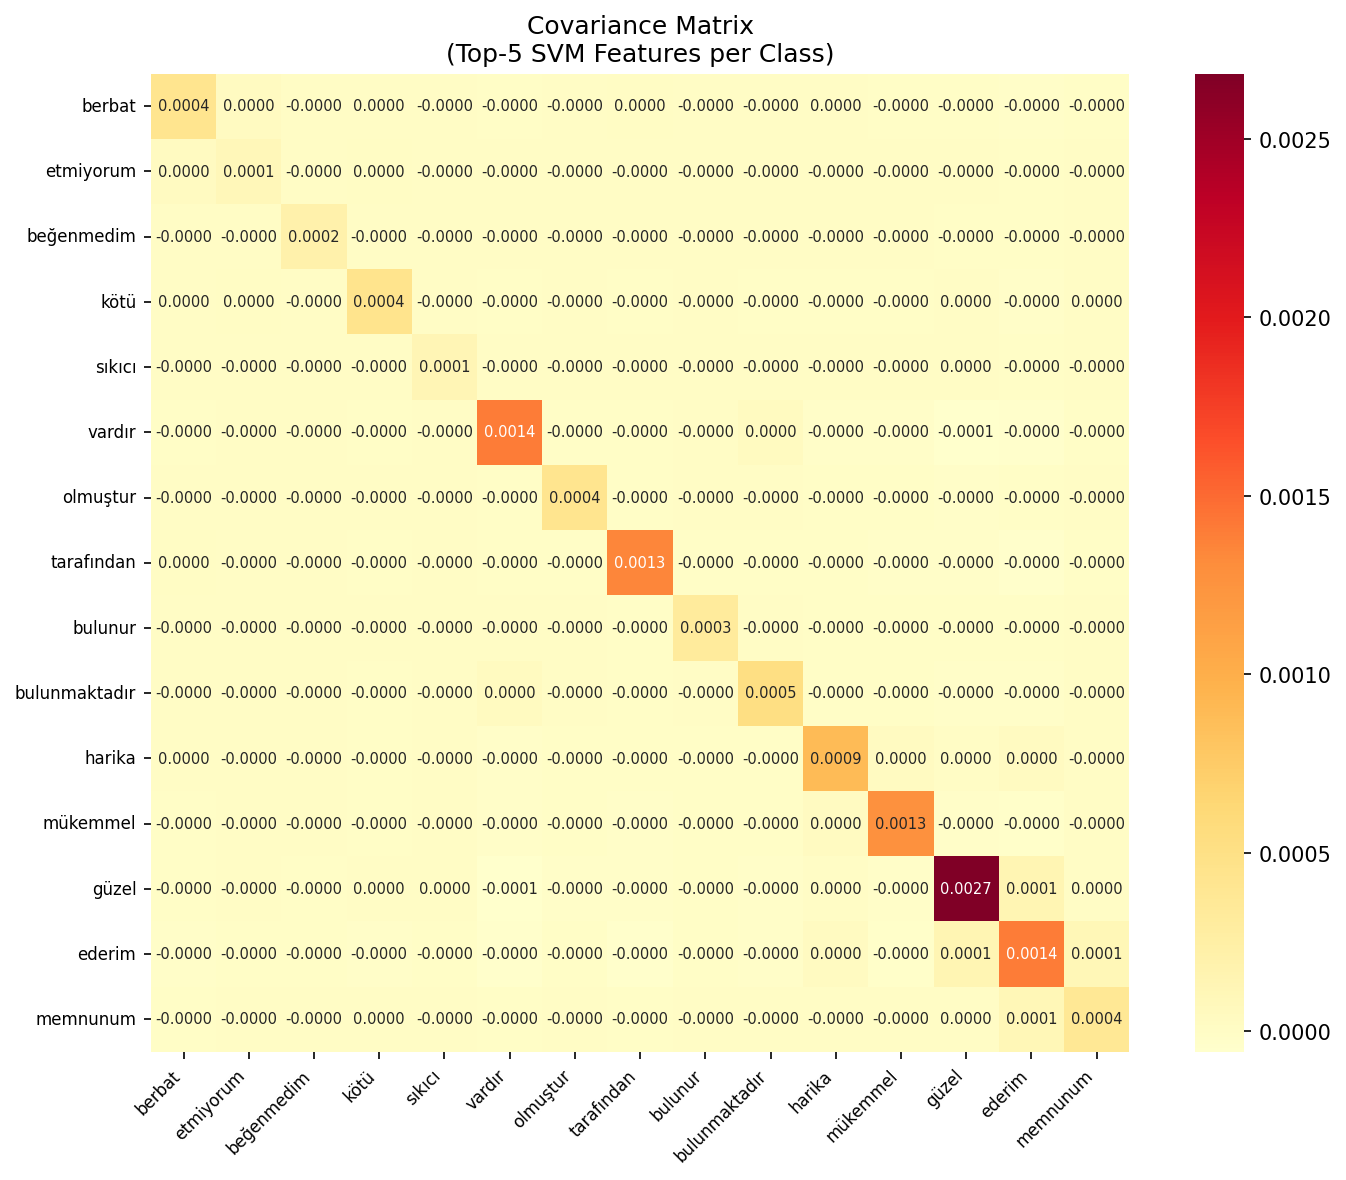
\includegraphics[width=\columnwidth]{turkish_sentiment/covariance_matrix.png}}
	\caption{Covariance matrix of the top-5 SVM features per class (15 features).
	         Near-diagonal structure confirms low feature co-variance in sparse TF-IDF space.}
	\label{fig:cov}
\end{figure}

\begin{figure}[htbp]
	\centerline{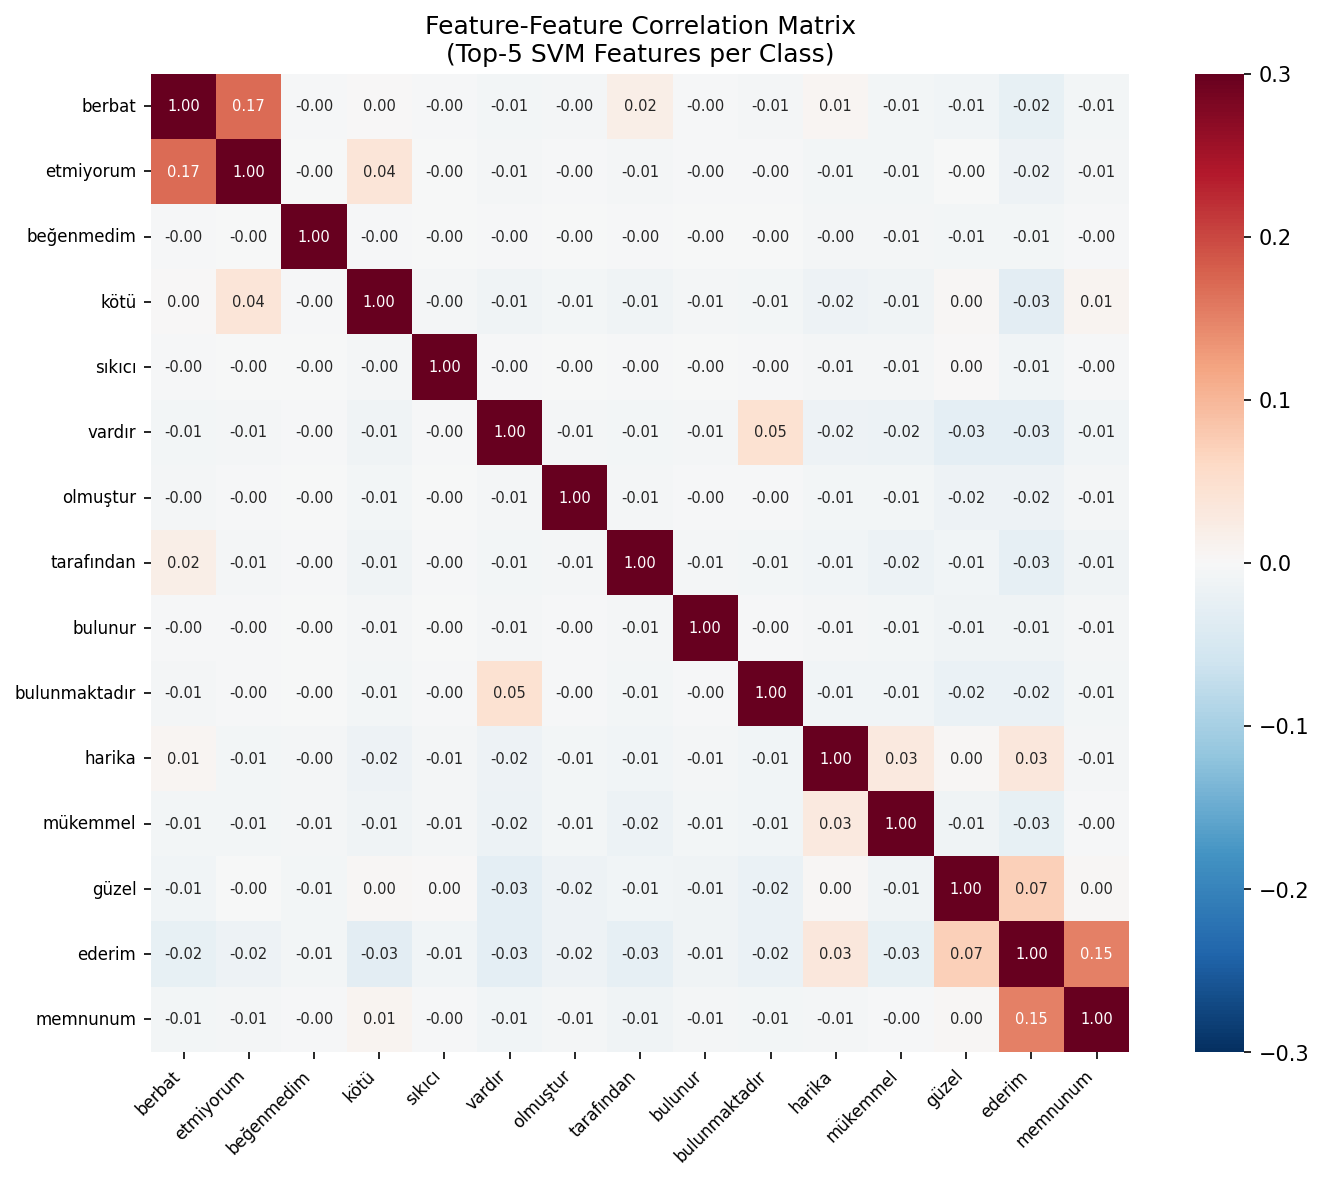
\includegraphics[width=\columnwidth]{turkish_sentiment/feature_correlation.png}}
	\caption{Pearson correlation matrix of the top-5 SVM discriminative features per class
	         (15 features). Near-zero off-diagonal values confirm feature independence in the
	         sparse TF-IDF space.}
	\label{fig:corr}
\end{figure}

\begin{table}[htbp]
	\caption{Top-10 Discriminative TF-IDF Features per Class (SVM coef\_)}
	\label{tab:top_features}
	\begin{center}
		\footnotesize
		\renewcommand{\arraystretch}{1.2}
		\setlength{\tabcolsep}{5pt}
		\begin{tabular}{lll}
			\toprule
			\rowcolor{headerblue}
			\color{white}\textbf{Pozitif} & \color{white}\textbf{Notr} & \color{white}\textbf{Negatif} \\
			\midrule
			\textit{harika}      & \textit{vardır}          & \textit{berbat}     \\
			\textit{mükemmel}    & \textit{olmuştur}        & \textit{etmiyorum}  \\
			\textit{güzel}       & \textit{tarafından}      & \textit{beğenmedim} \\
			\textit{ederim}      & \textit{bulunur}         & \textit{kötü}       \\
			\textit{memnunum}    & \textit{bulunmaktadır}   & \textit{sıkıcı}     \\
			\textit{gayet}       & \textit{değildir}        & \textit{iade}       \\
			\textit{1010}        & \textit{sahiptir}        & \textit{rezalet}    \\
			\textit{iyi}         & \textit{almıştır}        & \textit{en kötü}    \\
			\textit{teşekkürler} & \textit{aldı}            & \textit{yazık}      \\
			\textit{şık}         & \textit{genellikle}      & \textit{kalitesiz}  \\
			\bottomrule
		\end{tabular}
	\end{center}
\end{table}

\subsection{Data Clustering}

I also ran K-Means clustering (\texttt{random\_state=42}) on the PCA-50
representation and compared cluster assignments to true labels in Fig.~\ref{fig:kmeans}.
The Adjusted Rand Index is $\text{ARI} = -0.017$, showing that the TF-IDF feature
geometry does not support well-separated sentiment clusters. I expected this result:
in a bag-of-words representation, the same words can appear across different sentiment
contexts, so PCA space is not a reliable proxy for sentiment polarity. This is why I
chose supervised classifiers like SVM and LR, which optimize decision boundaries
directly rather than relying on cluster structure.

\begin{figure}[htbp]
	\centerline{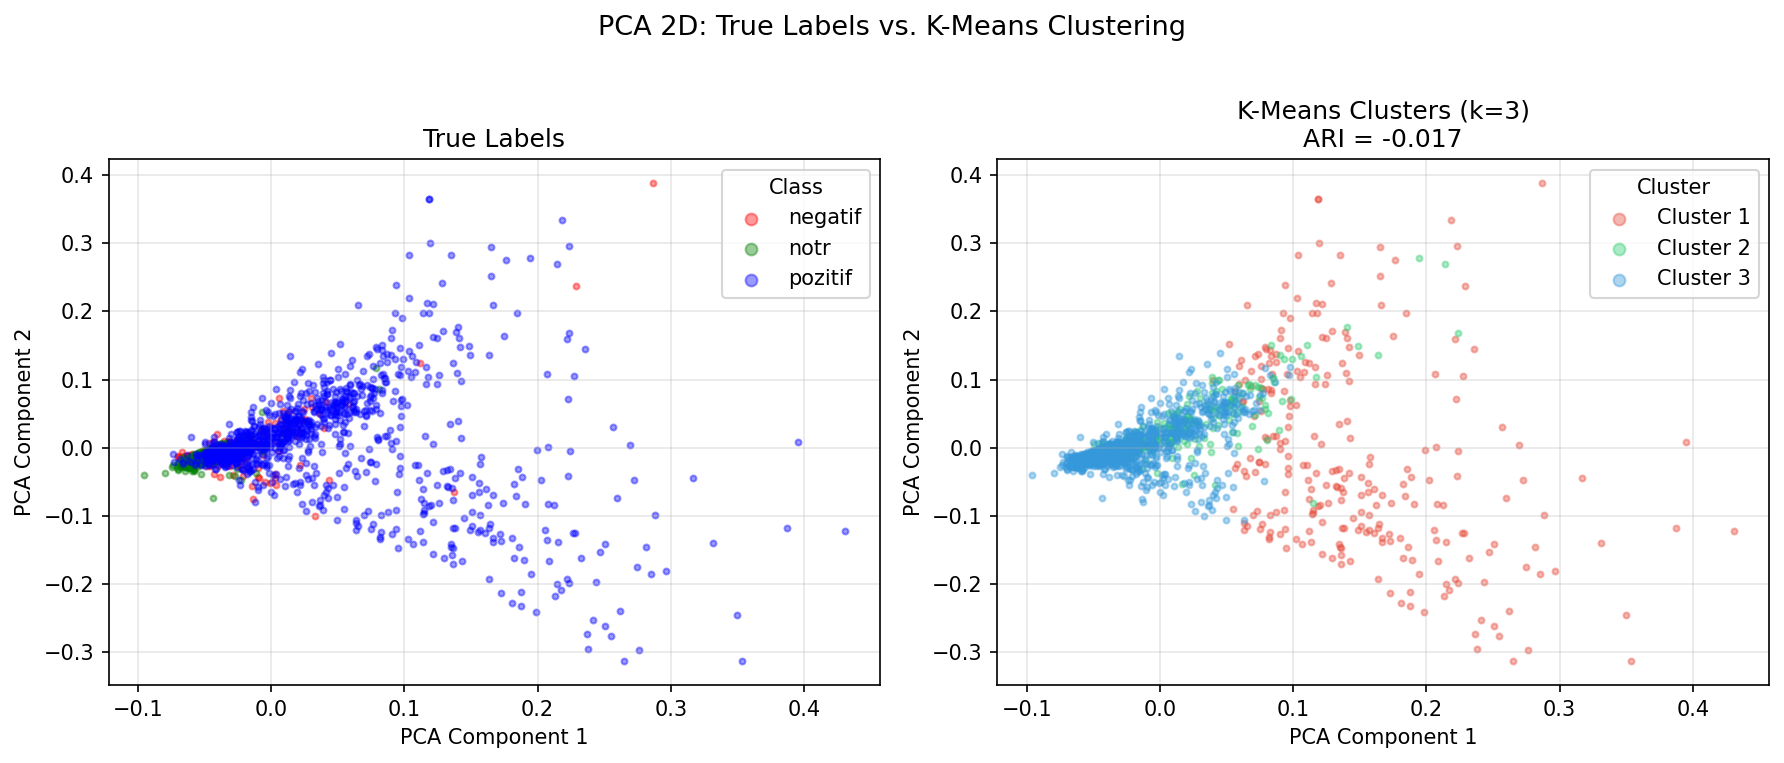
\includegraphics[width=\columnwidth]{turkish_sentiment/kmeans_clusters.png}}
	\caption{PCA-2D: true labels (left) vs.\ K-Means ($k=3$) clusters (right) on 2,000
	         test samples. ARI$=-0.017$ shows that sentiment classes do not form
	         geometrically separable clusters in TF-IDF PCA space.}
	\label{fig:kmeans}
\end{figure}

% ============================================================
\section{Models Used}
\label{sec:models}
% ============================================================

\subsection{Train/Validation/Test Split}

The dataset provides predefined train and test splits, which I used without modification.
I did not create a separate validation set. For training, I used a stratified 50,000-sample
subsample of the 440,679 training samples to keep experiment runtime feasible for all
models. For testing, I used a stratified 10,000-sample subset of the 48,965 test samples
(seed 42), preserving the original class ratios: 53.5\% pozitif, 34.9\% notr, 11.6\%
negatif. I did not apply strict 60/20/20 splits because the predefined splits ensure
comparability with published benchmarks; the 10-run experiment (Section~\ref{sec:results},
Table~\ref{tab:ttest}) with its internal 80/20 splits serves the role of cross-validation
for assessing model stability.

\subsection{Classical Pattern Classifiers}

I selected classifiers spanning different pattern recognition paradigms: probabilistic
(Naive Bayes), maximum-margin (SVM), linear probabilistic (Logistic Regression),
ensemble (Random Forest, XGBoost), instance-based (KNN), and single tree-based
(Decision Tree) to cover the full spectrum from simple to complex decision boundaries.
All use a TF-IDF pipeline with \texttt{norm='l2'}:

\textbf{Naive Bayes} (\texttt{MultinomialNB}, $\alpha=0.5$): Models each class as
a product of feature likelihoods. Simple and fast but assumes feature independence.

\textbf{SVM} (\texttt{LinearSVC}, $C=0.5$, \texttt{max\_iter=2000}): Finds the
maximum-margin hyperplane. Well-suited to high-dimensional sparse TF-IDF features.
Calibrated with \texttt{CalibratedClassifierCV} for probability output.

\textbf{Logistic Regression} (\texttt{saga} solver, $C=0.5$): A probabilistic linear
classifier. Competitive with SVM on text tasks and provides calibrated probabilities
natively.

\textbf{Random Forest} (200 trees, \texttt{max\_depth=None}): An ensemble of decision
trees using bootstrap sampling and feature bagging. More expressive than linear
models but slower on sparse TF-IDF.

\textbf{KNN} ($k=5$, \texttt{metric=cosine}): Classifies by majority vote among
$k$ nearest neighbors in TF-IDF space. No explicit training phase; sensitive to
document length normalization (handled by L2 norm).

\textbf{Decision Tree} (\texttt{max\_depth=20}, \texttt{criterion=gini}): A single
axis-aligned tree. Low computational cost but prone to overfitting in high-dimensional
sparse feature spaces; included to demonstrate the capacity mismatch with TF-IDF.

\textbf{XGBoost}~\cite{b_xgboost} (200 trees, \texttt{max\_depth=5}, \texttt{learning\_rate=0.05}):
Gradient-boosted trees. Strong on structured data; on sparse TF-IDF it is
slower than linear models and cannot leverage sparsity as effectively as SVM.

\subsection{Transformer Classifier (BERTurk)}

BERTurk (\texttt{dbmdz/bert-base-turkish-cased})~\cite{b7} is \textit{fully fine-tuned}
end-to-end for 3 epochs: all 12 transformer layers and the classification head are
updated during training (no frozen layers, no adapters, no LoRA). Training used
\texttt{learning\_rate=2e-5}, \texttt{batch\_size=32}, \texttt{max\_length=128},
\texttt{AdamW} optimizer with \texttt{warmup\_ratio=0.1} and \texttt{weight\_decay=0.01},
on an NVIDIA RTX~4060 Laptop GPU (8\,GB VRAM). BERTurk's WordPiece subword tokenizer
handles Turkish morphological variation without manual stemming or lemmatization.

% ============================================================
\section{Results}
\label{sec:results}
% ============================================================

\subsection{Evaluation Metrics}

I report Accuracy, Macro F1, and Macro ROC-AUC (one-vs-rest). Macro F1 is the
\textit{primary} metric because the dataset is imbalanced. It penalizes models that
ignore the minority \textit{negatif} class equally to those that fail on the majority
classes. ROC-AUC measures separability regardless of decision threshold.

\subsection{Confusion Matrices and Negatif Class Analysis}

Fig.~\ref{fig:cms} shows the confusion matrices for all eight models. The most important
pattern recognition challenge is the low recall for the \textit{negatif} class across
all models due to severe class imbalance (11.6\% of training data).

Table~\ref{tab:negatif_tp} quantifies this for the \textit{negatif} class
(support: 1,159 test samples). True Positives (TP), False Negatives (FN), False Positives
(FP), and True Negatives (TN) are derived from the confusion matrix rows and columns
corresponding to the negatif class.

\begin{table}[htbp]
	\caption{Negatif Class: TP, FN, FP, TN (test set, $n=10{,}000$)}
	\label{tab:negatif_tp}
	\begin{center}
		\footnotesize
		\renewcommand{\arraystretch}{1.2}
		\setlength{\tabcolsep}{5pt}
		\begin{tabular}{lrrrr}
			\toprule
			\rowcolor{headerblue}
			\color{white}\textbf{Model} & \color{white}\textbf{TP} & \color{white}\textbf{FN} & \color{white}\textbf{FP} & \color{white}\textbf{TN} \\
			\midrule
			Transformer      & 945 & 214 & 151 & 8690 \\
			SVM              & 757 & 402 & 132 & 8709 \\
			Naive Bayes      & 675 & 484 & 168 & 8673 \\
			Logistic Reg.    & 596 & 563 &  70 & 8771 \\
			Random Forest    & 435 & 724 &  72 & 8769 \\
			KNN              & 477 & 682 & 132 & 8709 \\
			XGBoost          & 465 & 694 & 105 & 8736 \\
			Decision Tree    & 433 & 726 & 267 & 8574 \\
			\bottomrule
		\end{tabular}
	\end{center}
\end{table}

The transformer recovers the most true negatives (TP=945, recall=81.5\%), reflecting
BERTurk's contextual understanding of negation. SVM achieves TP=757 (recall=65.3\%),
the best among classical models. Logistic Regression has the fewest false positives
(FP=70) at the cost of very low recall (FN=563). Decision Tree has the highest false
positive rate (FP=267) and the lowest recall alongside Random Forest, confirming
that axis-aligned splits cannot effectively model the negatif minority class in
high-dimensional TF-IDF space.

\begin{figure*}[htbp]
	\centerline{
\includegraphics[width=\textwidth]{turkish_sentiment/confusion_matrixes.png}}
	\caption{Confusion matrices for all 8 models on the Turkish Sentiment test set
	         ($n=10{,}000$). Rows = true class, columns = predicted class.
	         Classes: negatif (0), notr (1), pozitif (2). The negatif class (top row)
	         shows the most misclassification across all models.}
	\label{fig:cms}
\end{figure*}

\subsection{Model Comparison}

Table~\ref{tab:results} shows the main results for all eight models. BERTurk achieves
the best Macro-F1 of 0.9298 and ROC-AUC of 0.9909. SVM is the best classical model
(Macro-F1 = 0.8768, ROC-AUC = 0.9748), outperforming Naive Bayes by 2.8 F1 points and
Logistic Regression by 3.8 points. XGBoost (Macro-F1 = 0.7554) and Decision Tree
(Macro-F1 = 0.7063) are the weakest classical models: XGBoost's gradient boosting
cannot efficiently exploit TF-IDF sparsity, and Decision Tree's axis-aligned splits
collapse under high-dimensional feature pressure, yielding the largest gap between
Accuracy (0.7935) and Macro-F1 (0.7063) of any model. The transformer-to-SVM gap is
5.3 Macro-F1 points, larger than on balanced datasets (see Appendix~B), confirming
that class imbalance amplifies the transformer's contextual advantage.

\begin{table}[htbp]
	\caption{Turkish Sentiment Classification Results ($n=10{,}000$ test)}
	\label{tab:results}
	\begin{center}
		\footnotesize
		\renewcommand{\arraystretch}{1.2}
		\setlength{\tabcolsep}{5pt}
		\begin{tabular}{lccc}
			\toprule
			\rowcolor{headerblue}
			\color{white}\textbf{Model} & \color{white}\textbf{Accuracy} & \color{white}\textbf{Macro-F1} & \color{white}\textbf{ROC-AUC} \\
			\midrule
			\textbf{Transformer}     & \textbf{0.9574} & \textbf{0.9298} & \textbf{0.9909} \\
			SVM              & 0.9223 & 0.8768 & 0.9748 \\
			Naive Bayes      & 0.9062 & 0.8488 & 0.9670 \\
			Logistic Reg.    & 0.9048 & 0.8387 & 0.9735 \\
			Random Forest    & 0.8863 & 0.7893 & 0.9625 \\
			KNN              & 0.8622 & 0.7757 & 0.9217 \\
			XGBoost          & 0.8369 & 0.7554 & 0.9257 \\
			Decision Tree    & 0.7935 & 0.7063 & 0.8282 \\
			\bottomrule
		\end{tabular}
	\end{center}
\end{table}

Fig.~\ref{fig:overall} shows the model comparison bar chart across Accuracy, Macro-F1,
Precision, and Recall. The consistent gap between Accuracy and Macro-F1 (4.5 points
for SVM, 2.8 for Transformer) reflects the imbalance penalty. ROC curves are shown in
Fig.~\ref{fig:roc}.

\begin{figure*}[htbp]
	\centerline{
\includegraphics[width=\textwidth]{turkish_sentiment/overall.png}}
	\caption{Turkish Sentiment: Model performance comparison across Accuracy, Macro-F1,
	         Precision, and Recall. The gap between Accuracy and Macro-F1 is largest for
	         Random Forest (8.7 points) and smallest for Transformer (2.8 points).}
	\label{fig:overall}
\end{figure*}

\begin{figure*}[htbp]
	\centerline{
\includegraphics[width=\textwidth]{turkish_sentiment/roc_curves.png}}
	\caption{Turkish Sentiment: ROC-AUC curves (one-vs-rest per class). Transformer
	         macro AUC=0.991; SVM macro AUC=0.975. The negatif class (dashed lines)
	         shows consistently lower AUC than notr and pozitif across all models.}
	\label{fig:roc}
\end{figure*}

\subsection{Statistical Significance (10-Run Experiment)}

To validate that SVM's advantage over other classical classifiers is statistically
significant, I ran each model 10 times (seeds 0--9) on a stratified 10,000-sample
subsample of the training set (80/20 internal split per run), using the same TF-IDF
configuration. Table~\ref{tab:ttest} reports mean Macro-F1, standard deviation, and
two-sided independent t-test $p$-values comparing each model against SVM.

\begin{table}[htbp]
	\caption{10-Run Macro-F1: Mean $\pm$ Std and t-test vs.\ SVM}
	\label{tab:ttest}
	\begin{center}
		\footnotesize
		\renewcommand{\arraystretch}{1.2}
		\setlength{\tabcolsep}{6pt}
		\begin{tabular}{lccc}
			\toprule
			\rowcolor{headerblue}
			\color{white}\textbf{Model} & \color{white}\textbf{Mean F1} & \color{white}\textbf{Std} & \color{white}\textbf{$p$-value vs.\ SVM} \\
			\midrule
			SVM              & 0.8214 & 0.0057 &  \\
			Naive Bayes      & 0.8058 & 0.0070 & $<$0.0001 \\
			Logistic Reg.    & 0.7733 & 0.0083 & $<$0.0001 \\
			XGBoost          & 0.7539 & 0.0106 & $<$0.0001 \\
			KNN              & 0.7413 & 0.0083 & $<$0.0001 \\
			Random Forest    & 0.7360 & 0.0097 & $<$0.0001 \\
			Decision Tree    & 0.6751 & 0.0115 & $<$0.0001 \\
			\bottomrule
		\end{tabular}
	\end{center}
\end{table}

All $p$-values are below $0.0001$, confirming that SVM significantly outperforms every
other classical classifier across all seven models. Decision Tree shows the highest
variance ($\text{std}=0.0115$) and lowest mean F1 ($0.675$), consistent with its
overfitting tendency in high-dimensional sparse spaces. XGBoost ($0.754$) outperforms
Decision Tree and Random Forest but remains below the linear models, confirming that
gradient boosting cannot efficiently exploit TF-IDF sparsity. SVM's advantage stems
from three properties of LinearSVC: (1) it directly optimizes the margin in the
high-dimensional TF-IDF space where linear separability is good; (2) it is not sensitive
to feature independence assumptions (unlike Naive Bayes); and (3) L2 normalization
stabilizes the margin even under the unequal class distribution. The transformer was
excluded from the 10-run experiment due to GPU training cost ($\sim$33 minutes per run).

% ============================================================
\section{Conclusions}
\label{sec:conclusion}
% ============================================================

\textbf{What was accomplished.} I designed, trained, and evaluated a three-agent text
classification system using classical pattern recognition methods and BERTurk on Turkish
Sentiment Analysis. Across seven classical classifiers, SVM achieved the best classical
Macro-F1 (0.877 on the test set; 0.821 mean over 10 runs) and BERTurk achieved the best
overall result (Macro-F1 = 0.930). My 10-run statistical experiment confirmed SVM's
superiority over all classical alternatives ($p < 0.0001$).

\textbf{What was learned.} The key pattern recognition insight is that high-dimensional
sparse TF-IDF features provide a nearly linear feature space for sentiment classification,
which favors the maximum-margin approach of SVM. L2 normalization and linear decision
boundaries in a 30K-dimensional space are more effective than non-linear ensemble
methods (Random Forest, KNN) that cannot exploit global feature geometry. Class imbalance
(negatif: 11.6\%) is the primary challenge: even the transformer recovers only 81.5\%
of negatif instances. The K-Means ARI of $-0.017$ confirms that sentiment classes are
not geometrically separable in PCA space, reinforcing that supervised boundary
optimization (not cluster structure) drives performance.

\textbf{What could not be done.} Several things were outside my scope: (a) I did not
apply strict 60/20/20 splits, using predefined benchmark splits instead; (b) I did not
apply SMOTE or class-weighted loss to address negatif class under-representation;
(c) I chose hyperparameters manually from literature recommendations rather than
running a grid search; (d) I did not conduct quantitative evaluation of XAI faithfulness
(explanation stability, fidelity metrics).

\textbf{Future work.} Applying SMOTE or class-weighted LinearSVC to improve negatif
recall is the most impactful next step. Grid-search over SVM's $C$ parameter and TF-IDF
vocabulary size could close part of the transformer gap. Quantitative XAI faithfulness
evaluation (e.g., sufficiency and comprehensiveness metrics) would complete the pattern
recognition analysis beyond classification accuracy.

% ============================================================
\begin{thebibliography}{00}

\bibitem{b_duda}
R.~O.~Duda, P.~E.~Hart, and D.~G.~Stork,
\textit{Pattern Classification}, 2nd~ed.
New York, NY, USA: Wiley, 2001.

\bibitem{b2}
J.~Devlin, M.-W. Chang, K.~Lee, and K.~Toutanova,
``BERT: Pre-training of deep bidirectional transformers for language understanding,''
in \textit{Proc.\ NAACL-HLT},
Minneapolis, MN, USA, Jun.\ 2019, pp.~4171--4186.

\bibitem{b4}
S.~M.~Lundberg and S.-I.~Lee,
``A unified approach to interpreting model predictions,''
in \textit{Proc.\ NeurIPS},
Long Beach, CA, USA, Dec.\ 2017, pp.~4765--4774.

\bibitem{b5}
M.~T.~Ribeiro, S.~Singh, and C.~Guestrin,
```Why should I trust you?': Explaining the predictions of any classifier,''
in \textit{Proc.\ KDD},
San Francisco, CA, USA, Aug.\ 2016, pp.~1135--1144.

\bibitem{b7}
S.~Schweter,
``BERTurk: BERT models for Turkish,''
\textit{Zenodo}, Apr.\ 2020.
doi: 10.5281/zenodo.3770924.

\bibitem{b10}
S.~Minaee et al.,
``Deep learning--based text classification: A comprehensive review,''
\textit{ACM Comput.\ Surv.}, vol.~54, no.~3, pp.~1--40, Apr.\ 2021.

\bibitem{b_wj}
M.~Wooldridge and N.~R.~Jennings,
``Intelligent agents: Theory and practice,''
\textit{Knowl.\ Eng.\ Rev.}, vol.~10, no.~2, pp.~115--152, Jun.\ 1995.

\bibitem{b_trsentiment}
winvoker,
``Turkish Sentiment Analysis Dataset,''
Hugging Face Datasets, 2022.
[Online]. Available: \url{https://huggingface.co/datasets/winvoker/turkish-sentiment-analysis-dataset}

\bibitem{b_imdb}
stanfordnlp,
``Large Movie Review Dataset (IMDB),''
Hugging Face Datasets, 2022.
[Online]. Available: \url{https://huggingface.co/datasets/stanfordnlp/imdb}

\bibitem{b_agnews}
sh0416,
``AG's News Topic Classification Dataset,''
Hugging Face Datasets, 2023.
[Online]. Available: \url{https://huggingface.co/datasets/sh0416/ag_news}

\bibitem{b_trnews}
S.~Aras,
``TTC4900: A Benchmark Data for Turkish Text Categorization,''
Hugging Face Datasets, 2022.
[Online]. Available: \url{https://huggingface.co/datasets/savasy/ttc4900}

\bibitem{b_xgboost}
T.~Chen and C.~Guestrin,
``XGBoost: A scalable tree boosting system,''
in \textit{Proc.\ KDD},
San Francisco, CA, USA, Aug.\ 2016, pp.~785--794.

\bibitem{b_tsne}
L.~van~der~Maaten and G.~Hinton,
``Visualizing data using t-SNE,''
\textit{J.\ Mach.\ Learn.\ Res.}, vol.~9, pp.~2579--2605, Nov.\ 2008.

\bibitem{b_tfidf}
G.~Salton and C.~Buckley,
``Term-weighting approaches in automatic text retrieval,''
\textit{Inf.\ Process.\ Manag.}, vol.~24, no.~5, pp.~513--523, 1988.

\end{thebibliography}

% ============================================================
\appendix
\section{Code Repository}
\label{appendix:code}
% ============================================================

The full source code, dataset configuration files, experiment scripts, and all figures
for this project are available at:

\begin{center}
  \href{https://github.com/oruccakir/multi-agent-xai-text-classifier}{https://github.com/oruccakir/multi-agent-xai-text-classifier}
\end{center}

The repository is organised as follows: \texttt{src/} contains training and evaluation
pipelines; \texttt{agents/} contains the three-agent routing logic; \texttt{app/}
contains the Streamlit interface; \texttt{reports/} contains this document and all
generated figures; \texttt{scripts/} contains figure generation scripts for this report.

% ============================================================
\section{Additional Dataset Results}
\label{appendix:datasets}
% ============================================================

Table~\ref{tab:appendix_summary} summarises results for the three additional datasets
used in this project. Full confusion matrices, ROC curves, and per-model figures are
available in the GitHub repository.

\begin{table}[htbp]
	\caption{Additional Datasets: Best Classical Model and Transformer Macro-F1}
	\label{tab:appendix_summary}
	\begin{center}
		\footnotesize
		\renewcommand{\arraystretch}{1.3}
		\setlength{\tabcolsep}{4pt}
		\begin{tabular}{lllcc}
			\toprule
			\rowcolor{headerblue}
			\color{white}\textbf{Dataset} & \color{white}\textbf{Task} & \color{white}\textbf{Best Classical} & \color{white}\textbf{F1-M} & \color{white}\textbf{Transformer F1-M} \\
			\midrule
			IMDB           & Bin. Sentiment & SVM    & 0.895 & 0.907 \\
			AG News        & 4-class Topics & SVM    & 0.915 & 0.928 \\
			Turkish News   & 7-class Topics & SVM    & 0.919 & 0.938 \\
			\bottomrule
		\end{tabular}
	\end{center}
\end{table}

\textbf{Cross-dataset patterns.} SVM is the best classical model on all three datasets.
The transformer-to-SVM gap is 1.2--1.9 F1 points on balanced datasets, much smaller
than the 5.3-point gap on Turkish Sentiment. This confirms that class imbalance amplifies
the transformer's advantage. Decision Tree collapses on multi-class tasks (AG News
F1=0.611, Turkish News F1=0.491), while KNN performs competitively on short text
(Turkish News F1=0.884).

\end{document}
